\chapter{Quantum computing}
\label{chap:quantum}
The field of quantum computing is split in two main branches: the development of quantum hardware and the study of algorithms that use such hardware.
Only the second branch is relevant for this thesis, and even so only a brief explanation is offered here.
This chapter is primarily based on the Qiskit textbook \cite{qiskit_textbook} and \citetitle{textbook_2nd} by \textcite{textbook_2nd}.
The discussion of variational quantum algorithms in section \ref{sec:vqa} is based on the review by \textcite{cerezo2021}.
\section{The qubit}
The quantum bit, the qubit, is the building block of quantum computing.
Like the classical binary digit it can be either 0 or 1.
But being quantum, these are quantum states, $\ket{0}$ and $\ket{1}$, and the qubit can be in any superposition of these states.
The state of the qubit lies in a two-dimensional Hilbert space, and the states $\ket{0}$ and $\ket{1}$ are basis vectors, known as the computational basis states.
Thus, the state of a qubit can be expressed as
\begin{equation}
  \ket{\psi} = \alpha \ket{0} + \beta \ket{1} = \begin{pmatrix} \alpha \\ \beta \end{pmatrix}
  \label{eq:qubit}
\end{equation}
where $\alpha$ and $\beta$ are any numbers, even complex ones.
The only requirement is that the state is normalised, i.e., $\vert\alpha\vert^2 + \vert\beta\vert^2 = 1$.

Normalisation is required due to the Born rule, as the absolute square of the coefficients is the probability of measuring the qubit in the corresponding basis state.
It is one of nature's great mysteries what exactly a measurement is, but in the quantum computational setting, it can be thought of as taking a random sample with the probabilities given by the coefficients, which can be done systematically.

\subsection{The Bloch sphere}
A useful tool for visualising the state of a qubit is the Bloch sphere.
First, it should be noted for states on the form \cref{eq:qubit} are not unique, only the relative complex phase matters.
There is a global phase which is not measurable, and thus not relevant for the state of the qubit.
Therefore, taking also the normalisation requirement into account, the state of the qubit can be expressed as
\begin{equation}
  \ket{\psi} = \cos\left(\frac{\theta}{2}\right) \ket{0} + e^{i\phi} \sin\left(\frac{\theta}{2}\right) \ket{1}
  \label{eq:bloch}
\end{equation}
where $\theta, \phi \in \mathbb{R}$.
Interpreting $\theta$ as the polar angle and $\phi$ the azimuthal angle, the state of the qubit can be identified with a point a sphere, the Bloch sphere.
There, the state $\ket{0}$ is typically thought of as the north pole, and $\ket{1}$ as the south pole.
\Cref{fig:bloch} shows the Bloch sphere, and the state of the qubit in \cref{eq:bloch}.

% insert figure place holder
\begin{figure}
  \centering
  \def\svgwidth{0.4\textwidth}
  %% Creator: Inkscape 1.2.1 (9c6d41e, 2022-07-14), www.inkscape.org
%% PDF/EPS/PS + LaTeX output extension by Johan Engelen, 2010
%% Accompanies image file 'bloch_sphere.pdf' (pdf, eps, ps)
%%
%% To include the image in your LaTeX document, write
%%   \input{<filename>.pdf_tex}
%%  instead of
%%   \includegraphics{<filename>.pdf}
%% To scale the image, write
%%   \def\svgwidth{<desired width>}
%%   \input{<filename>.pdf_tex}
%%  instead of
%%   \includegraphics[width=<desired width>]{<filename>.pdf}
%%
%% Images with a different path to the parent latex file can
%% be accessed with the `import' package (which may need to be
%% installed) using
%%   \usepackage{import}
%% in the preamble, and then including the image with
%%   \import{<path to file>}{<filename>.pdf_tex}
%% Alternatively, one can specify
%%   \graphicspath{{<path to file>/}}
%% 
%% For more information, please see info/svg-inkscape on CTAN:
%%   http://tug.ctan.org/tex-archive/info/svg-inkscape
%%
\begingroup%
\makeatletter%
\providecommand\color[2][]{%
  \errmessage{(Inkscape) Color is used for the text in Inkscape, but the package 'color.sty' is not loaded}%
  \renewcommand\color[2][]{}%
}%
\providecommand\transparent[1]{%
  \errmessage{(Inkscape) Transparency is used (non-zero) for the text in Inkscape, but the package 'transparent.sty' is not loaded}%
  \renewcommand\transparent[1]{}%
}%
\providecommand\rotatebox[2]{#2}%
\newcommand*\fsize{\dimexpr\f@size pt\relax}%
\newcommand*\lineheight[1]{\fontsize{\fsize}{#1\fsize}\selectfont}%
\ifx\svgwidth\undefined%
  \setlength{\unitlength}{177.93310547bp}%
  \ifx\svgscale\undefined%
    \relax%
  \else%
    \setlength{\unitlength}{\unitlength * \real{\svgscale}}%
  \fi%
\else%
  \setlength{\unitlength}{\svgwidth}%
\fi%
\global\let\svgwidth\undefined%
\global\let\svgscale\undefined%
\makeatother%
\begin{picture}(1,1.06027363)%
  \lineheight{1}%
  \setlength\tabcolsep{0pt}%
  \put(0,0){\includegraphics[width=\unitlength,page=1]{bloch_sphere.pdf}}%
  \put(0.2887321,0.28921972){\color[rgb]{0,0,0}\makebox(0,0)[lt]{\lineheight{0}\smash{\begin{tabular}[t]{l}$x$\\ \end{tabular}}}}%
  \put(0.97157299,0.44096214){\color[rgb]{0,0,0}\makebox(0,0)[lt]{\lineheight{0}\smash{\begin{tabular}[t]{l}$y$\end{tabular}}}}%
  \put(0.45522726,0.9935414){\color[rgb]{0,0,0}\makebox(0,0)[lt]{\lineheight{0}\smash{\begin{tabular}[t]{l}$z$\end{tabular}}}}%
  %\put(0.44047452,0.41690636){\color[rgb]{0,0,0}\makebox(0,0)[lt]{\lineheight{0}\smash{\begin{tabular}[t]{l}φ\end{tabular}}}}%
  \put(0.44047452,0.41690636){\color[rgb]{0,0,0}\makebox(0,0)[lt]{\lineheight{0}\smash{\begin{tabular}[t]{l}$\phi$\end{tabular}}}}%
  % \put(0.45101219,0.69597371){\color[rgb]{0,0,0}\makebox(0,0)[lt]{\lineheight{0}\smash{\begin{tabular}[t]{l}θ\end{tabular}}}}%
  \put(0.45101219,0.69597371){\color[rgb]{0,0,0}\makebox(0,0)[lt]{\lineheight{0}\smash{\begin{tabular}[t]{l}$\theta$\end{tabular}}}}%
  \put(0,0){\includegraphics[width=\unitlength,page=2]{bloch_sphere.pdf}}%
  \put(0.04935377,0.94994952){\color[rgb]{0,0,0}\makebox(0,0)[lt]{\lineheight{0}\smash{\begin{tabular}[t]{l} \end{tabular}}}}%
  % \put(0,0){\includegraphics[width=\unitlength,page=3]{figs/bloch/bloch_sphere.pdf}}%
  \put(0.46622932,0.0080449){\color[rgb]{0,0,0}\makebox(0,0)[lt]{\lineheight{0}\smash{\begin{tabular}[t]{l}$\ket{1}$\end{tabular}}}}%
  % \put(0,0){\includegraphics[width=\unitlength,page=4]{figs/bloch/bloch_sphere.pdf}}%
  \put(0.35242254,0.95312728){\color[rgb]{0,0,0}\makebox(0,0)[lt]{\lineheight{0}\smash{\begin{tabular}[t]{l}$\ket{0}$\end{tabular}}}}%
  % \put(0,0){\includegraphics[width=\unitlength,page=5]{figs/bloch/bloch_sphere.pdf}}%
  % \put(0.6104334,0.7732887){\color[rgb]{0,0,0}\makebox(0,0)[lt]{\lineheight{0}\smash{\begin{tabular}[t]{l}ψ\end{tabular}}}}%
  \put(0.6104334,0.7732887){\color[rgb]{0,0,0}\makebox(0,0)[lt]{\lineheight{0}\smash{\begin{tabular}[t]{l}$\ket{\psi}$\end{tabular}}}}%
\end{picture}%
\endgroup%

  \caption{
    The Bloch sphere in which a qubit state is represented by a point.
    The state $\ket{0}$ is the north pole, and $\ket{1}$ is the south pole.
    The angle $\theta$ is the polar angle, determining the probability of measuring the qubit in the state $\ket{0}$, while the azimuthal angle $\phi$ corresponds to the complex phase.
    From \cite{wikipedia_bloch}.
  }
  \label{fig:bloch}
\end{figure}

\subsection{Multiple qubits}
Although the continuous nature of the qubit is indeed useful, the true power of quantum computers lie in how multiple qubits interact.
Having multiple qubits allows for the creation of entanglement, which is a key feature of quantum computing.

With just two qubits, there are four possible states, $\ket{00}, \ket{01}, \ket{10}, \ket{11}$.
Each of these four have their own probability amplitude, and thus their own probability of being measured.
A two-qubit system will therefore operate on with four complex numbers.

Generally, the state of multiple qubits can be expressed using the tensor product as
\begin{equation}
  \ket{\psi_1 \psi_2 \cdots  \psi_n} = \ket{\psi_1} \otimes \ket{\psi_2} \otimes \cdots \otimes \ket{\psi_n}
  \label{eq:tensor}.
\end{equation}
What makes this so powerful is that the state of a multi-qubit system can be anything on the form
\begin{equation}
  \ket{\psi_1 \psi_2 \cdots  \psi_n}
  = c_1 \ket{0\dots 00} + c_2 \ket{0\dots 01} + \cdots + c_{2^n} \ket{1\dots 11}
  = \begin{pmatrix}
    c_1 \\ c_2 \\ \vdots \\ c_{2^n}
  \end{pmatrix}
  \in \mathbb{C}^{2^n},
  \label{eq:superposition}
\end{equation}
which means that with $n$ qubits, the system can be in any superposition of the $2^n$ basis states.
Operating on several qubits then, one can do linear algebra in an exponentially large space.

\section{Operating with qubits}
\subsection{Single-qubit gates}
To operate on one or more qubits, a unitary operation is applied to the state, where the unitarity is needed for states to remain normalised.
With the finite number of qubits, these operations can be expressed as matrices.
These operations are often thought of as gates, paralleling the classical gates in digital logic.
The most basic gates are the Pauli gates, which are the $X$, $Y$ and $Z$ gates:
\begin{align}
  X =\ket{0}\bra{1} + \ket{1}\bra{0} & = \begin{pmatrix} 0 & 1 \\ 1 & 0 \end{pmatrix},  \\
  Y =\ket{0}\bra{1} - \ket{1}\bra{0} & = \begin{pmatrix} 0 & -i \\ i & 0 \end{pmatrix}, \\
  Z =\ket{0}\bra{0} - \ket{1}\bra{1} & = \begin{pmatrix} 1 & 0 \\ 0 & -1 \end{pmatrix}.
\end{align}
These gates can be seen as half turns around the $x$, $y$ and $z$ axes, respectively, of the Bloch sphere.
The $X$ gate is also known as the NOT gate, as it mirrors the classical NOT gate by mapping $\ket{0}$ to $\ket{1}$ and vice versa, though it of course is more general, being applicable to superposition states too.

The Hadamard gate
\begin{equation}
  H = \frac{1}{\sqrt{2}} \begin{pmatrix} 1 & 1 \\ 1 & -1 \end{pmatrix}
\end{equation}
is a rotation around the $x$-axis by $\pi/2$.
It is a very important gate in quantum computing, as it is used to create superpositions of the computational basis states.


The $R_X$, $R_Y$ and $R_Z$ gates are rotations around the $x$, $y$ and $z$ axes, respectively, by an arbitrary angle $\theta$:
\begin{align*}
  R_X(\theta) & = \begin{pmatrix} \cos\left(\frac{\theta}{2}\right) & -i \sin\left(\frac{\theta}{2}\right) \\ -i \sin\left(\frac{\theta}{2}\right) & \cos\left(\frac{\theta}{2}\right) \end{pmatrix}, \\
  R_Y(\theta) & = \begin{pmatrix} \cos\left(\frac{\theta}{2}\right) & -\sin\left(\frac{\theta}{2}\right) \\ \sin\left(\frac{\theta}{2}\right) & \cos\left(\frac{\theta}{2}\right) \end{pmatrix},      \\
  R_Z(\theta) & = \begin{pmatrix} e^{-i\frac{\theta}{2}} & 0 \\ 0 & e^{i\frac{\theta}{2}} \end{pmatrix}.
\end{align*}
These parametrised gates will be useful in \cref{sec:vqa}.

\subsection{Multi-qubit gates}
The most important multi-qubit gate is the controlled-$X$ gate, also known as the CNOT, which is a controlled version of the $X$ gate.
Being controlled means that it only acts on the second qubit if the first qubit is in the state $\ket{1}$.
Of course, the first qubit may be in a superposition, and the CNOT this way allows for the creation of entanglement between the two qubits.
If the first qubit has probability amplitude $\alpha$ of being in the state $\ket{1}$, the second qubit will have probability amplitude $\alpha$ of being flipped.
The CNOT gate can be expressed in matrix form as
\begin{equation}
  \text{CNOT} = \begin{pmatrix} 1 & 0 & 0 & 0 \\ 0 & 1 & 0 & 0 \\ 0 & 0 & 0 & 1 \\ 0 & 0 & 1 & 0 \end{pmatrix}.
\end{equation}

\subsection{Observables and measurements}
For an output to be obtained from a quantum computer, a measurement must be performed.
This is typically done at the end of all operations and of all qubits, thus yielding a single output of zeroes and ones, a bit-string.
It is important to note that the measurement is not a deterministic process, but rather a probabilistic one.
Often, the underlying probabilities are what is of interest.
Therefore, many measurements are performed.
Usually, these results are averaged to obtain an estimate, but more complicated post-processing methods are also possible.
For instance, neural networks have shown useful properties in regard of reducing variance in the estimates, though at the cost of some bias \cite{torlai2020}.

The $Z$ basis is the canonical basis for measurements, but any other basis can be used, at least in theory.
Often, only canonical basis measurements are implemented in the hardware.
Using another basis can be done by properly preparing the state before the measurement.

Measurements may be done in the middle of operations and be used to control the operations.
If the qubits are entangled, measuring one can affect the measurement probabilities of others.
Using such intermediate measurements is a way of introducing non-linearities in the otherwise unitary nature of the quantum world.


\subsection{Quantum circuits}
The operations on qubits are often described using quantum circuits, which are a graphical representation of the operations on the qubits, the quantum algorithms.
They are read from left to right.
It is standard procedure to assume all qubits start in the state $\ket{0}$.
Gates are generally written as boxes with the name of the gate insides.
An example is the circuit
\begin{equation}
  \begin{quantikz}
    \lstick{$\ket{0}$} & \gate{H} & \ctrl{1} & \qw \\
    \lstick{$\ket{0}$} & \qw & \targ{} & \qw
  \end{quantikz}
\end{equation}
in which the first qubit is put into a superposition using the Hadamard gate before a CNOT gate is applied to the second, controlled on the first.
This creates the state $\frac{1}{\sqrt{2}}\left(\ket{00} + \ket{11}\right)$.

\section{Limitations of NISQ hardware}
Quantum hardware have been physically realised and even outperforms classical computers in very contrived situations, but the hardware is still very limited.
The hardware is limited in the number of qubits, the connectivity between the qubits, and the noise and decoherence of the qubits.
It is believed that quantum hardware will continue to improve and eventually perform demanding algorithms like Shor's for large numbers.
Still, the era dubbed NISQ (Noisy Intermediate-Scale Quantum) is the first step, and to make use of the hardware, algorithms must take these limitations into consideration.

Noise and decoherence severely limits how large circuits can be run on the hardware.
Decoherence refers to the fact that the qubits are not isolated from the environment, and may be ruined by the environment, e.g., electrical noise from the control electronics.
Furthermore, with the continuous nature of quantum states, minor errors can compound.
If for instance a qubit is to be rotated many times, a small error in the rotation may cause the qubit to be rotated by a large angle.
Because of this, NISQ algorithms must be shallow, meaning that the amount of gates applied before measurement is small.

Another limiting factor is the amount of qubits.
Current hardware has around 10-100 qubits, which though still may be enough to express states too large to be expressed on classical computers, is not enough to perform the most demanding algorithms.
With more qubits, error correction could be used to mitigate the effects of noise and decoherence, but this would require many more qubits than are currently available.
Another current limitation is the connectivity between the qubits.
Not all qubits are directly linked, which means that applying a multi-qubit gate may require intermediate swapping of qubits.
This increases circuit depth which in turn increases the error rate.

\section{Variational quantum algorithms}
\label{sec:vqa}
Variational quantum algorithms (VQAs) are envisioned as the most likely candidate for quantum advantage to be achieved.
By optimising a set of parameters that describe the quantum circuit, classical optimisation techniques are applicable, and only using the quantum hardware for what can be interpreted as function calls, limits the circuit depths needed.
Running the same circuit many times with slightly different parameters and inputs in a classical-quantum-hybrid fashion, rather than a complete quantum implementation, means that the quantum operations can be simple enough for the noise and decoherence to be manageable.

Generally, VQAs start with defining a cost function, depending on some input data (states) and the parametrised circuit, to be minimised with respect to the parameters of the quantum circuit.
For example, the cost function for the variational quantum eigensolver (VQE) is the expectation value of some Hamiltonian, which is the energy of a system.
The cost function should be meaningful in the sense that the minimum coincides with the optimal solution to the problem, and that lower values generally implies better solutions.
Additionally, the cost function should be complicated enough to warrant quantum computation by not being easily calculated on classical hardware, while still having few enough parameters to be efficiently optimised.

The optimisation of the cost function is often done with gradient descent methods.
To evaluate the gradient of the quantum circuit with respect to the parameters, the very convenient parameter shift rule is often used.
Though appearing almost as a finite difference scheme, relying on evaluating the circuit with slightly shifted parameters, it is indeed an exact formula.
Furthermore, it may be used recursively to evaluate higher order derivatives, which allows usage of more advanced optimisation methods like the Newton method that require the Hessian.

VQA's applications are numerous.
A typical example is finding the ground state of a Hamiltonian for a molecule.
Such problems are exponential in the particle count, and thus intractable on classical hardware for larger molecules, while the problem of evaluating the Hamiltonian on quantum hardware is typically polynomial.
VQAs are also well suited for general mathematical problems and optimisation, with another common example being QAOA for the max-cut problem.

Still, there are many difficulties when applying VQAs.
Exponentially vanishing gradients, known as barren plateaus, are a common occurrence, making the optimisation futile.
The choosing of the ansatz determines the performance and feasibility of the algorithms, and there are many strategies and options.
Some rely on exploiting the specific quantum hardware's properties, while other use the specifics of the problem at hand.
Finally, the inherent noise and errors on near-term hardware will still be a problem and limit circuit depths.
